\documentclass[a4paper]{spie}  % A4; compressed in-text cites [4,5]

\renewcommand{\baselinestretch}{1.0}

% Checklist A4 side margins: 1.93 cm (spie.cls a4paper patch is commented out)
\oddsidemargin -0.61cm
\evensidemargin -0.61cm

\usepackage{times}
\usepackage{mathptmx}  % Times math (rsfs installed)
\usepackage{amsmath,amsfonts,amssymb}
\usepackage{graphicx}
\usepackage{booktabs,multirow,adjustbox}
\usepackage{float}
\usepackage[table]{xcolor}
\usepackage{soul}
\usepackage[hidelinks]{hyperref}
% Shared table colors/macros. \input this from main.tex PREAMBLE after:
%   \usepackage{booktabs,multirow,adjustbox}
%   \usepackage[table]{xcolor}
\definecolor{color_gray}{RGB}{229,229,229}
\definecolor{color_blue}{RGB}{252,182,165}
\definecolor{color_pink}{RGB}{255,217,178}
\definecolor{color_yellow}{RGB}{255,255,204}
\definecolor{color_blue1}{RGB}{135,206,235}
\newcommand{\sidelabel}[2]{%
  \multirow{#1}{*}{\rotatebox[origin=c]{90}{\scalebox{0.95}{\scriptsize #2}}}%
}


% Dual PDF: set \SynGSHighlighttrue for yellow revision marks; omit/false for clean.
\newif\ifSynGSHighlight
%\SynGSHighlighttrue
\sethlcolor{yellow}
\soulregister{\cite}{1}
\soulregister{\textbf}{1}
\soulregister{\emph}{1}
\soulregister{\textit}{1}
\soulregister{\textsuperscript}{1}
% Do not soulregister \ref — it breaks \hl/\rev (infinite expansion).
\ifSynGSHighlight
  \newcommand{\rev}[1]{\hl{#1}}
\else
  \newcommand{\rev}[1]{#1}
\fi

% Checklist: superscript [n] / [4,5] wrapping the whole cite list
\renewcommand{\citeform}[1]{#1}
\renewcommand{\citepunct}{,}
\makeatletter
\AtBeginDocument{%
  \def\@citess#1{\mbox{$\m@th^{\hbox{\OverciteFont{[#1]}}}$}}%
}
\makeatother
\renewcommand{\Authsep}{, }
\renewcommand{\Authands}{, and }

\title{SynGS: Synergizing explicit geometry and transformer depth priors for sparse-view 3D Gaussian Splatting}

\author[a]{Junjie Geng*}%
\author[a]{Ao Zhang}%
\author[a]{Bo Zhang}%
\author[a]{Lian Duan}
\affil[a]{Communication University of China, State Key Laboratory of Media Convergence and Communication, Intelligent Network and Media Research Center, No. 1 Dingfuzhuang East Street, Chaoyang District, Beijing 100024, China}

\authorinfo{*J.G.: E-mail: gjj@cuc.edu.cn\\
A.Z.: E-mail: 2212433186@qq.com}

\pagestyle{empty}

\begin{document}
\maketitle

\begin{abstract}
In 360-degree scenes captured with sparse views, 3D Gaussian Splatting (3DGS) reconstruction is susceptible to the loss of edge detail, geometric instability in occluded regions, and overfitting to foreground regions. \rev{To address the reconstruction difficulties arising from limited input observations, we introduce SynGS, which incorporates explicit geometric constraints and depth information into the 3D Gaussian Splatting framework.} The proposed method leverages the visual hull to impose explicit geometric constraints and integrates a Transformer-based depth prior to facilitate global cross-view consistency, complemented by a geometry enhancement pipeline. By combining reliable depth filtering with fine-grained structural detail recovery and incorporating a dynamic visibility regularization strategy, our approach enables adaptive reweighting of supervision signals during optimization. \rev{The experimental findings indicate favorable PSNR and SSIM results for SynGS. In the Mip-NeRF 360 experiments, its PSNR and SSIM values exceed those reported for the selected baseline methods under the evaluated input-view configurations,} reaching 25.91~dB in PSNR and 0.948 in SSIM using only four input views. On LLFF, the improvements are more apparent in the four- and six-view settings, while the nine-view results remain comparable to those of other evaluated methods.
\end{abstract}

\keywords{~Novel View Synthesis, 3D Gaussian Splatting, Few-shot reconstruction, Geometry Prior-Guided Reconstruction, Vision Transformer}

\section{INTRODUCTION}
\label{sec:intro}

Sparse inputs provide limited information about visible regions, causing 3D reconstruction methods to overfit local observations and struggle to maintain global geometric consistency~\cite{Yang23_FreeNeRF}. Sparse observations also introduce greater geometric ambiguity, making occluded regions, textureless areas, and view boundaries prone to missing geometry, structural distortions, and degraded appearance~\cite{Niemeyer22_RegNeRF}. \rev{Kerbl et al.}~\cite{Kerbl23_3DGS} \rev{proposed 3D Gaussian Splatting (3DGS), which achieves fast training and real-time rendering through a tile-based rasterization mechanism. Subsequent developments have further enhanced the representation through structured Gaussian organization}~\cite{Lu24_ScaffoldGS}. Under sparse views, Structure-from-Motion (SfM)~\cite{Schonberger16_COLMAP} often recovers incomplete point clouds. Since 3DGS relies on SfM cameras and sparse points for initialization, weak coverage harms geometric convergence~\cite{Chung24_DepthRegGS}. Limited cross-view constraints further cause floaters and pseudo-geometry~\cite{Xu25_DropoutGS}, while sparse supervision~\cite{Park25_DropGaussian} and visibility imbalance aggravate overfitting~\cite{Somraj23_ViPNeRF}.

Existing sparse-view methods have explored depth regularization~\cite{Li24_DNGaussian}, Gaussian densification~\cite{Zhu24_FSGS}, co-regularization~\cite{Zhang24_CoRGS}, and Gaussian dropout~\cite{Park25_DropGaussian} to improve reconstruction. Nevertheless, incomplete initial geometry and overfitting during optimization remain challenges when only a few observations are available. \rev{To mitigate these challenges, we develop SynGS within the sparse-view 3DGS setting, where geometry-guided Gaussian initialization is coupled with regularization during training.} By strengthening initial geometric support and mitigating overfitting during optimization, SynGS improves reconstruction robustness under severely limited view coverage.
The main contributions are:
\begin{itemize}
\item \textbf{Visual Hull Initialization.} We incorporate a visual hull derived from multi-view silhouettes to provide an explicit geometric constraint for Gaussian initialization. This constraint complements incomplete SfM observations and helps establish a more reliable initial spatial distribution of Gaussian primitives.
\item \textbf{VGGT-Guided Densification.} We develop a pre-optimization densification strategy that back-projects cross-view-consistent depth estimates from VGGT to supplement the sparse initial point set. By introducing additional geometric samples before training, this strategy improves geometric coverage in under-observed regions.
\item \textbf{Dynamic Visibility Regularization.} We incorporate Dynamic Visibility Regularization during training to stochastically mask Gaussian primitives, redistribute optimization gradients, and mitigate overfitting under limited-view supervision. \rev{Together with the geometry-enhanced initialization, this regularization contributes to more robust reconstruction when only a limited number of input views are available.}
\end{itemize}

% Related Work — SPIE: section titles ALL CAPS; citations via \cite{}
\section{RELATED WORK}
\label{sec:related}

\rev{In neural rendering, Neural Radiance Fields (NeRF) employ an implicit radiance field representation, allowing high-quality images of unseen viewpoints to be synthesized through differentiable rendering}~\cite{Mildenhall21_NeRF}. Under sparse views, however, insufficient observations cause severe geometric ambiguity. Depth-guided approaches further improve structural consistency~\cite{Wang23_SparseNeRF}, while other methods constrain unobserved regions~\cite{Niemeyer22_RegNeRF}. \rev{In contrast to implicit radiance field representations, 3D Gaussian Splatting (3DGS) models scenes explicitly using optimizable Gaussian primitives, with differentiable rasterization supporting efficient training and real-time rendering}~\cite{Kerbl23_3DGS}. Beyond the original formulation, structured Gaussian representations improve robustness and view-adaptive rendering~\cite{Lu24_ScaffoldGS}. Depth-based approaches introduce additional geometric supervision~\cite{Li24_DNGaussian}, while densification-based methods improve Gaussian coverage~\cite{Zhu24_FSGS}. Other strategies include epipolar depth priors~\cite{Zheng25_NexusGS}. Others explore co-regularization~\cite{Zhang24_CoRGS} and Gaussian dropout~\cite{Park25_DropGaussian}.

\rev{Monocular depth estimators provide useful cues for underconstrained views}~\cite{Yang24_DepthAnythingV2}. Although depth supervision, Gaussian densification, and training-time regularization have improved sparse-view reconstruction, limited-view observations can still result in incomplete initial geometry and overfitting during optimization. To address these challenges, SynGS combines explicit visual-hull constraints with a VGGT-based multi-view depth prior~\cite{Wang25_VGGT} to augment the initial Gaussian geometry before optimization, and incorporates Dynamic Visibility Regularization during training to alleviate sparse-view overfitting.

% Method — SPIE section title ALL CAPS; subsections in separate files
\section{METHOD}
\label{sec:method}

\subsection{Overall Framework}
\label{sec:overall}

\rev{SynGS is developed as a sparse-view 3D Gaussian Splatting}~\cite{Kerbl23_3DGS} \rev{framework that combines explicit geometric initialization, depth-guided point cloud densification, and visibility-aware optimization.} Figure~\ref{fig:framework} \rev{illustrates the overall pipeline, which takes sparsely captured images and their corresponding foreground masks as input.} While recent variants organize Gaussians with structured scaffolds~\cite{Lu24_ScaffoldGS}, SynGS focuses on silhouette-based initialization and depth-guided densification under sparse posed inputs.

\begin{figure}[ht]
\centering
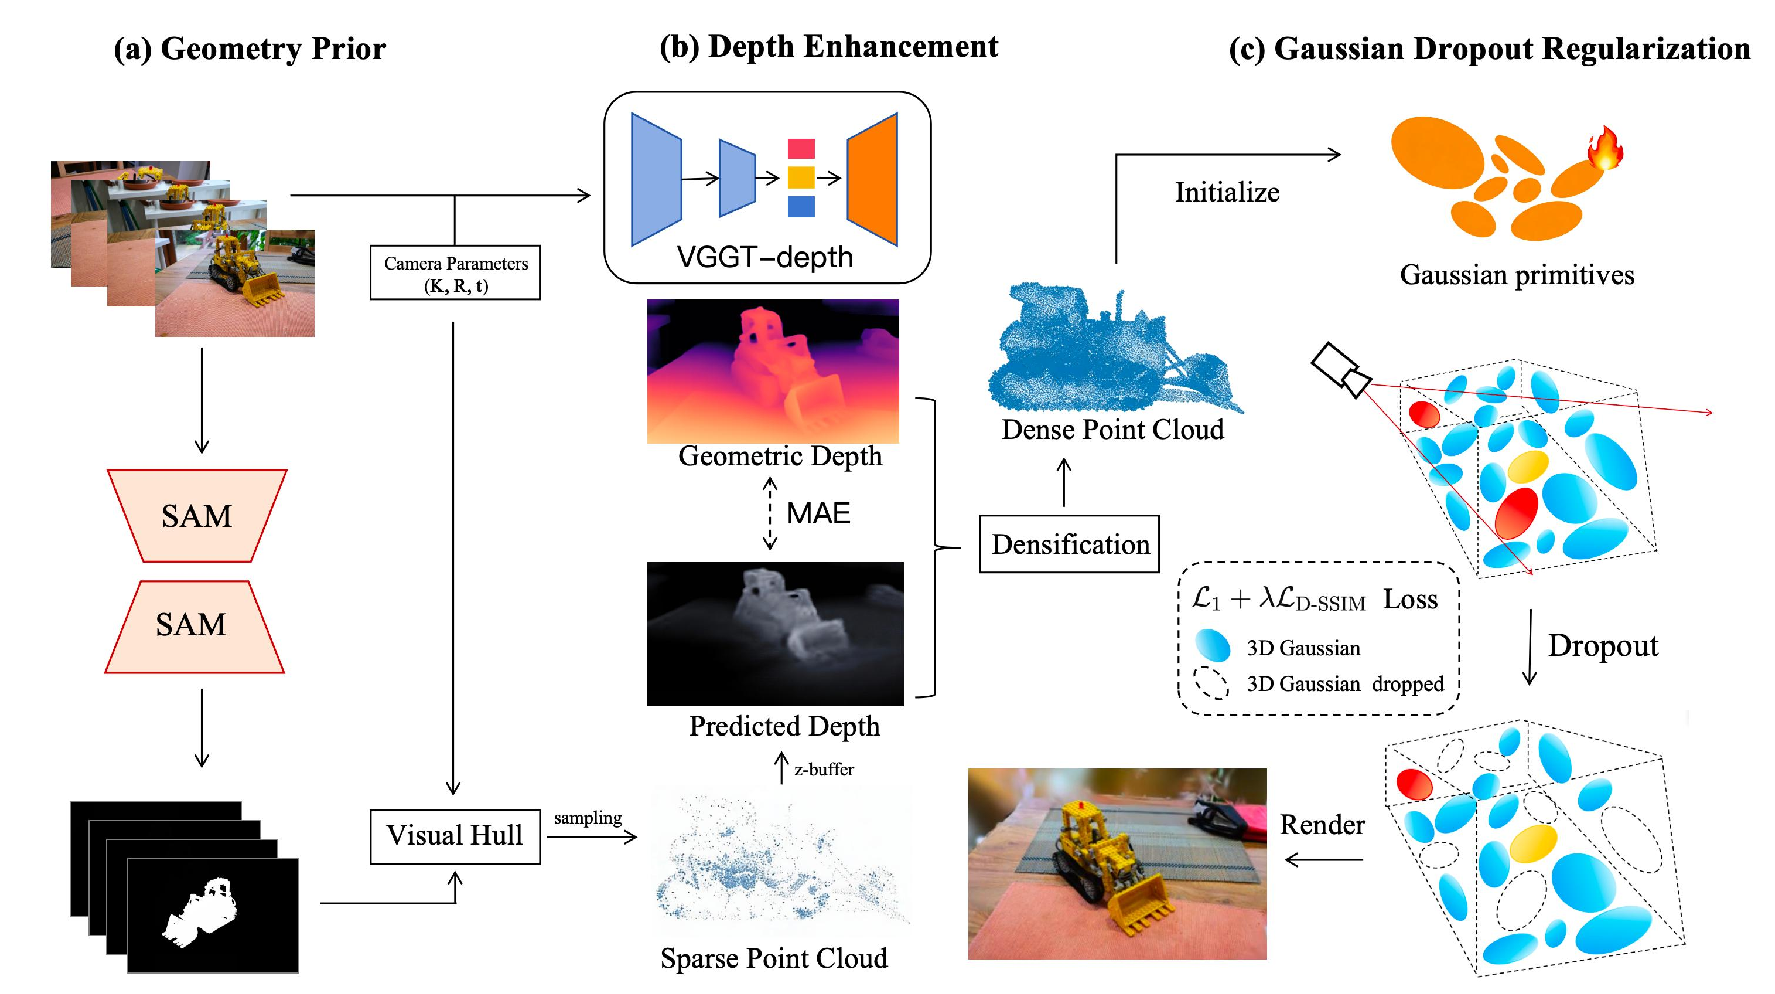
\includegraphics[width=0.90\textwidth]{figures/framework.pdf}
\caption{\label{fig:framework} Overview of the SynGS pipeline. The third stage applies Dynamic Visibility Regularization (DVR).}
\end{figure}

First, \textbf{Visual Hull Initialization} constructs a coarse geometric prior from multi-view silhouettes and generates an initial point cloud. Then, \textbf{VGGT-Guided Densification} exploits cross-view depth priors to supplement missing geometry and produce a depth-enhanced point cloud for Gaussian initialization. Finally, \textbf{Dynamic Visibility Regularization (DVR)} is applied during 3DGS optimization to rebalance supervision under sparse visibility and reduce overfitting. The complete process proceeds from the Visual Hull point cloud, through depth densification and Gaussian initialization, to DVR-regularized optimization.

\subsection{Visual Hull Initialization}
\label{sec:visual_hull}

Under sparse views, Structure-from-Motion (SfM)~\cite{Schonberger16_COLMAP} often produces sparse and incomplete point clouds. Weak coverage then destabilizes 3DGS optimization. We construct a Visual Hull prior from sparse multi-view images, camera parameters, and foreground masks, with light mask cleanup at boundaries. With known cameras, silhouettes are back-projected into 3D, and multi-view silhouette consistency defines a coarse geometric envelope of the target~\cite{Laurentini94_VisualHull}.

Candidate points are retained only when their projections agree with all valid foreground masks, then cleaned by one-time statistical and radius-based outlier filtering. The scaffold is stable but coarse: silhouette-based reconstruction cannot fully recover concave regions and fine structures. Sec.~\ref{sec:depth_densify} supplements the missing geometry before Gaussian initialization.

\subsection{VGGT-Guided Densification}
\label{sec:depth_densify}

Silhouettes alone miss concave regions and fine structures. We densify the Visual Hull point cloud with \textbf{VGGT-Depth}: from a pre-trained VGGT backbone~\cite{Wang25_VGGT}, a depth prior adaptation branch with cross-attention over multi-view tokens and a lightweight fusion head predicts per-view depth and confidence. Unlike a frozen monocular depth network~\cite{Yang24_DepthAnythingV2}, the adaptation branch is conditioned on multi-view tokens (Figure~\ref{fig:vggt_depth}).

\begin{figure}[ht]
\centering
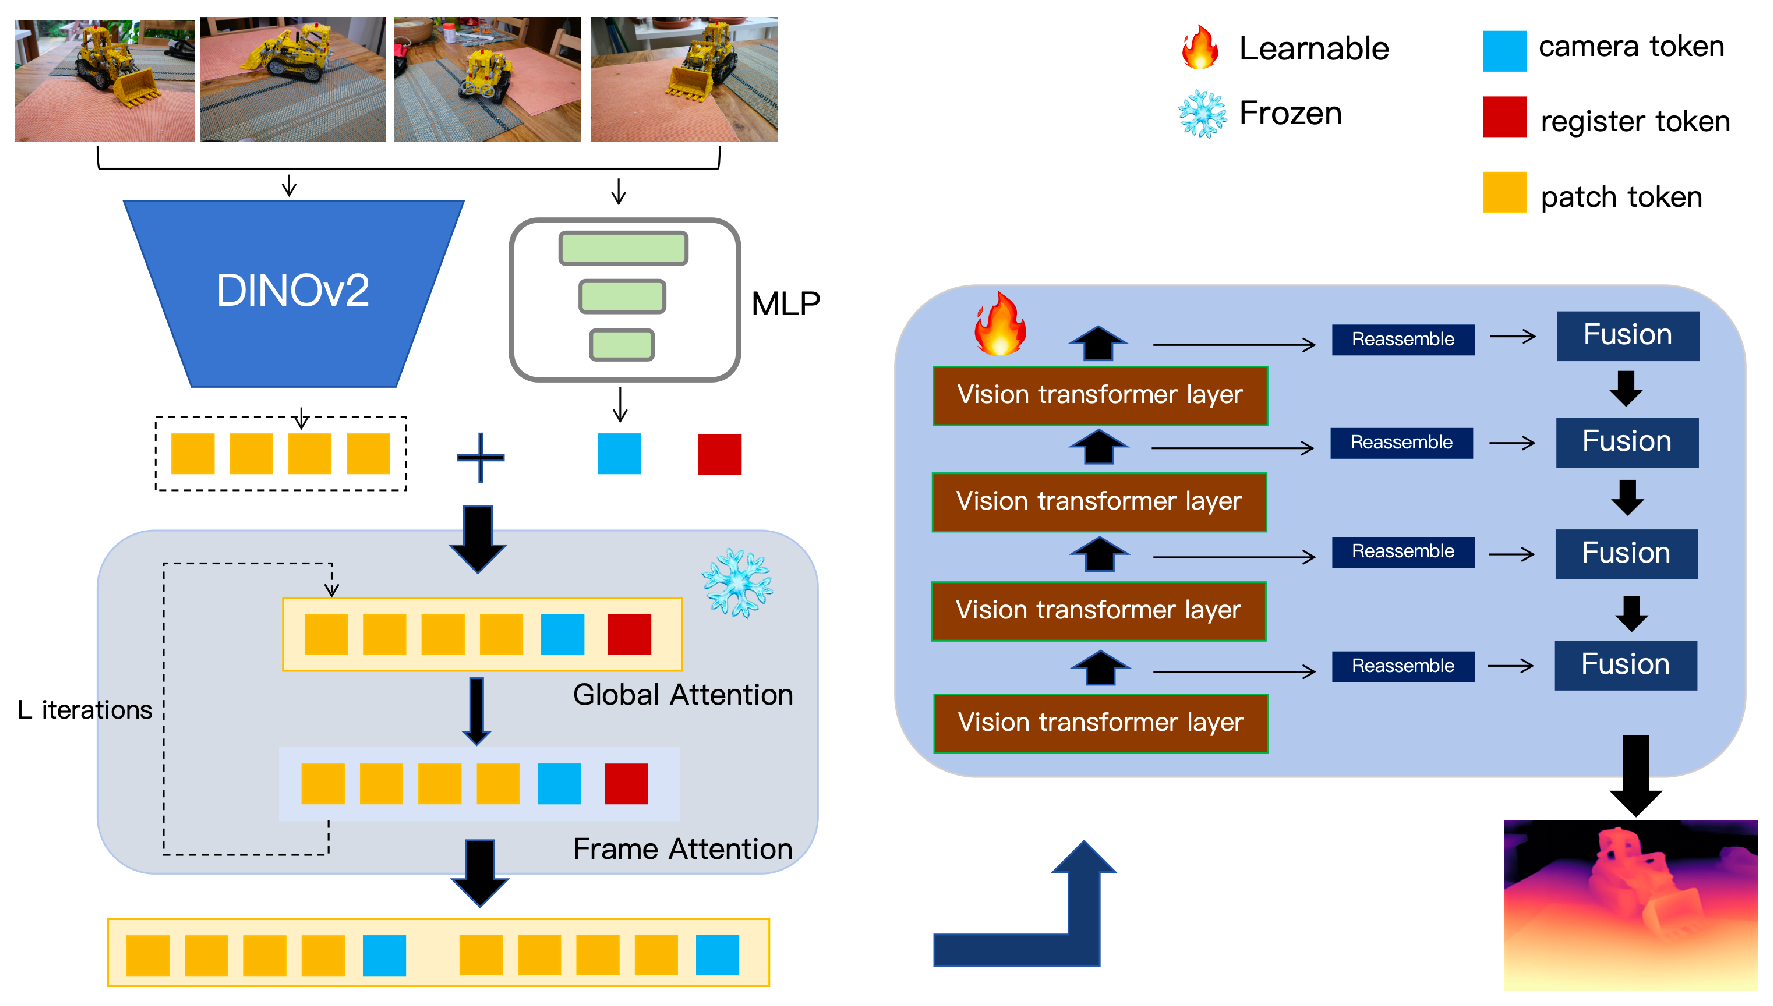
\includegraphics[width=0.90\textwidth]{figures/vggt_depth.pdf}
\caption{\label{fig:vggt_depth} VGGT-Depth prior used for depth-guided point cloud densification.}
\end{figure}

We use the Visual Hull AABB diagonal $L$ as the scene-scale reference. For each view, masked depth MAE against dataset ground-truth depth is used only to filter views and rays during densification (not at inference or when computing metrics); it is normalized by the 95th percentile over validation views to obtain $q_v$. Views with $q_v<0.4$ are discarded. If fewer than $0.8N$ views remain, densification is skipped and the Visual Hull point cloud is retained. Remaining views keep regions that pass VGGT-Depth confidence and depth consistency. With tolerance
\begin{equation}
\label{eq:delta_d}
\Delta(d)=\alpha d+\beta,\qquad
\alpha=0.01,\quad \beta=0.002L,
\end{equation}
we reject low-confidence or inconsistent observations before back-projection.

Point supplementation runs only along reliable rays. For each point, the top $K=3$ reliable views are selected; candidates are sampled around the predicted depth and back-projected. Here supplementation is applied offline to the Visual Hull point cloud before training. Complementary work injects epipolar depth priors into sparse-view Gaussian reconstruction~\cite{Zheng25_NexusGS}; we instead use adapted VGGT-Depth predictions for back-projection. Supplementary points are merged via two-stage voxel fusion and deduplication ($0.01L$ then $0.004L$).

\rev{Each densified point defines a Gaussian center, whose scale is initialized using the mean distance to its $k=8$ nearest neighbors. Color information from multiple views is combined using weights derived from depth consistency and VGGT confidence.} Opacity is set from cross-view consistency and clipped to $[0.2,0.8]$. Uneven supervision remains under sparse views; we address this with DVR (Sec.~\ref{sec:dvr}).

\rev{The initialization procedure separates the construction of the initial geometric support from the subsequent optimization of Gaussian attributes. Silhouette consistency first establishes the spatial envelope, whereas depth-based supplementation adds samples in regions that the initial representation may not describe adequately. These operations are completed before the Gaussian optimization stage. Consequently, the following regularization stage operates on an initialized representation that already incorporates the accepted geometric samples.}

\subsection{Dynamic Visibility Regularization}
\label{sec:dvr}

Sparse-view optimization remains strongly visibility-dependent. Distant, occluded, or poorly observed Gaussians appear in fewer views or pixels and receive weaker reconstruction gradients~\cite{Xu25_DropoutGS,Park25_DropGaussian}. Visibility priors have also been explored to regularize sparse-input radiance fields~\cite{Somraj23_ViPNeRF}. We use DVR via progressive Gaussian dropout.

At iteration $t$, DVR randomly masks a subset of Gaussians for dropout rendering. The dropout ratio grows linearly:
\begin{equation}
\label{eq:dropout_ratio}
r_t=\min\left(r_{\max},\,\gamma\frac{t}{T}\right),
\end{equation}
where $t$ and $T$ are the current and total iterations, $r_{\max}$ is the maximum dropout ratio, and $\gamma=0.1$--$0.2$ controls the growth rate. Early training keeps weak dropout for geometric convergence; later training increases it against sparse-view overfitting.

Used alone, random dropout can induce opacity or scale compensation; we keep a full-render branch as an anchor. Unlike compensated rendering that rescales retained primitives~\cite{Park25_DropGaussian}, the dropout branch is left uncompensated, while the full set is rendered in parallel under the same target. \rev{Let $I_{\mathrm{full}}$ and $I_{\mathrm{drop}}$ represent the renderings obtained with and without Gaussian dropout, respectively, and let $I$ denote the ground-truth image. The color loss is defined as:}
\begin{equation}
\label{eq:color_loss}
\mathcal{L}_{\mathrm{color}}(\hat{I},I)
=
(1-\lambda)\,\mathcal{L}_{1}(\hat{I},I)
+
\lambda\,\mathcal{L}_{\mathrm{D\text{-}SSIM}}(\hat{I},I),
\end{equation}
with $\lambda=0.2$~\cite{Kerbl23_3DGS}. The final objective is
\begin{equation}
\label{eq:dvr_loss}
\mathcal{L}
=
\mathcal{L}_{\mathrm{color}}(I_{\mathrm{full}},I)
+
\beta\,\mathcal{L}_{\mathrm{color}}(I_{\mathrm{drop}},I),
\end{equation}
where $\beta=0.5$--$1.0$. Related sparse-view designs further modulate masking with depth and density cues~\cite{Song26_D2GS}; DVR instead uses a progressive random schedule with an uncompensated dropout branch.


% Experiments — SPIE section title ALL CAPS; subsections in separate files
\section{EXPERIMENTS}
\label{sec:experiments}

\subsection{Experimental Setup and Datasets}
\label{sec:setup}

We evaluate SynGS on Mip-NeRF 360 (unbounded 360$^{\circ}$ scenes)~\cite{Barron22_MipNeRF360} and LLFF (forward-facing real captures)~\cite{Mildenhall19_LLFF}. All images are downsampled by a factor of 8. Mip-NeRF 360 scenes are tested with 4, 6, and 9 uniformly sampled input views. Metrics are PSNR, SSIM, and LPIPS. We compare SynGS with the NeRF- and 3DGS-based methods listed in Tables~\ref{tab:mip360} and~\ref{tab:llff}.

Training follows the standard 3DGS framework. Depth priors come from VGGT-Depth. Consistent with Sec.~\ref{sec:depth_densify}, view- and ray-level selection during densification may use dataset ground-truth depth only as a filter; novel-view rendering and all reported metrics do not use ground-truth depth. The model is trained for 30K iterations, with 3DGS initialization optimized for 10K iterations. Floaters are periodically removed during training. Experiments use PyTorch on an NVIDIA RTX 4090 GPU.

\subsection{Quantitative and Qualitative Results}
\label{sec:results}

% Table 1 — paste full numbers from the manuscript; do not invent values
% Table 1 — data from latex/MipNeRF360数据集/formatting-instructions-latex.tex (unchanged numbers)
\begin{table}[ht!]
\centering
\caption{\label{tab:mip360} \rev{Sparse-view results on Mip-NeRF 360 (4/6/9 views). LPIPS$^{*}$ denotes LPIPS $\times 10^{2}$.}}
\setlength{\tabcolsep}{2.8mm}
\renewcommand{\arraystretch}{1.08}
\adjustbox{width=1\linewidth}{%
\begin{tabular}{c l | ccc | ccc | ccc}
\toprule
\multirow{2}{*}{}
  & \multirow{2}{*}{Methods}
  & \multicolumn{3}{c|}{Mip-NeRF 360 (4-view)}
  & \multicolumn{3}{c|}{Mip-NeRF 360 (6-view)}
  & \multicolumn{3}{c}{Mip-NeRF 360 (9-view)} \\
&
  & LPIPS$^{*}$$\downarrow$ & PSNR$\uparrow$ & SSIM$\uparrow$
  & LPIPS$^{*}$$\downarrow$ & PSNR$\uparrow$ & SSIM$\uparrow$
  & LPIPS$^{*}$$\downarrow$ & PSNR$\uparrow$ & SSIM$\uparrow$ \\
\midrule
\sidelabel{2}{NeRF-based}
  & RegNeRF
      & 19.88 & 12.59 & 0.841
      & 20.72 & 13.41 & 0.847
      & 19.70 & 13.68 & 0.852 \\
  & SparseNeRF
      & 17.76 & 12.83 & 0.845
      & 19.74 & 13.42 & 0.861
      & 21.56 & 14.36 & 0.873 \\
\addlinespace[4pt]
\sidelabel{5}{3DGS-based}
  & 3DGS
      &10.80 & 20.31 & 0.899
      &8.38 & 22.12 & 0.913
      &6.42 & 24.29 & 0.930 \\
  & CoR-GS
      &11.76 & 20.45 & 0.856
      &9.28 & 22.57 & 0.901
      &7.04 & 24.73 & 0.926 \\
  & DropGaussian
      &11.57 & 21.76 & 0.837
      &8.61 & 22.98 & 0.895
      &8.02 & 24.10 & 0.915 \\
  & D$^2$GS
      &\cellcolor{color_blue}2.58 &\cellcolor{blue!8}22.35 &\cellcolor{blue!8}0.923
      &\cellcolor{color_blue}2.34 &\cellcolor{blue!8}24.74 &\cellcolor{blue!8}0.937
      &\cellcolor{color_blue}2.11 &\cellcolor{blue!8}27.13 &\cellcolor{blue!8}0.941 \\
  & SynGS (Ours)
      &\cellcolor{blue!8}3.89 &\cellcolor{color_blue}25.91 &\cellcolor{color_blue}0.948
      &\cellcolor{blue!8}3.43 &\cellcolor{color_blue}27.93 &\cellcolor{color_blue}0.953
      &\cellcolor{blue!8}3.02 &\cellcolor{color_blue}29.21 &\cellcolor{color_blue}0.961 \\
\bottomrule
\end{tabular}%
}
\end{table}

% Table 2 — data from latex/FFLL数据集/formatting-instructions-latex.tex (unchanged numbers)
\begin{table}[ht!]
\centering
\caption{\label{tab:llff} \rev{Sparse-view results on LLFF (4/6/9 views). LPIPS$^{*}$ denotes LPIPS $\times 10^{2}$.}}
\setlength{\tabcolsep}{2.8mm}
\renewcommand{\arraystretch}{1.08}
\adjustbox{width=1\linewidth}{%
\begin{tabular}{c l | ccc | ccc | ccc}
\toprule
\multirow{2}{*}{}
  & \multirow{2}{*}{Methods}
  & \multicolumn{3}{c|}{LLFF (4-view)}
  & \multicolumn{3}{c|}{LLFF (6-view)}
  & \multicolumn{3}{c}{LLFF (9-view)} \\
&
  & LPIPS$^{*}$$\downarrow$ & PSNR$\uparrow$ & SSIM$\uparrow$
  & LPIPS$^{*}$$\downarrow$ & PSNR$\uparrow$ & SSIM$\uparrow$
  & LPIPS$^{*}$$\downarrow$ & PSNR$\uparrow$ & SSIM$\uparrow$ \\
\midrule
\sidelabel{2}{NeRF-based}
  & RegNeRF
      & 29.65 & 18.55 & 0.587
      & 22.61 & 19.08 & 0.760
      & 18.39 & 22.86 & 0.820 \\
  & FreeNeRF
      & 30.85 & 19.09 & 0.624
      & 23.06 & 19.81 & 0.763
      & 17.94 & 23.08 & 0.823 \\
\addlinespace[4pt]
\sidelabel{5}{3DGS-based}
  & 3DGS
      &22.93 & 19.32 & 0.649
      &13.45 & 23.80 & 0.814
      &9.68 & 25.44 & 0.860 \\
  & CoR-GS
      &19.66 & 20.45 & 0.696
      &\cellcolor{color_blue}12.53 & 23.87 & 0.840
      &\cellcolor{color_blue}8.94 & 26.70 &\cellcolor{color_blue}0.874 \\
  & DropGaussian
      &21.93 & 19.80 & 0.621
      &13.79 & 23.41 & 0.803
      &9.40 & 25.87 & 0.868 \\
  & D$^2$GS
      &\cellcolor{blue!8}17.98 &\cellcolor{blue!8}22.35 &\cellcolor{blue!8}0.746
      &13.85 &\cellcolor{blue!8}23.91 &\cellcolor{blue!8}0.846
      &8.91 &\cellcolor{color_blue}26.80 &\cellcolor{blue!8}0.871 \\
  & SynGS (Ours)
      &\cellcolor{color_blue}16.92 &\cellcolor{color_blue}23.92 &\cellcolor{color_blue}0.762
      &\cellcolor{blue!8}12.54 &\cellcolor{color_blue}25.17 &\cellcolor{color_blue}0.848
      &\cellcolor{blue!8}8.96 &\cellcolor{blue!8}26.71 &\cellcolor{blue!8}0.871 \\
\bottomrule
\end{tabular}%
}
\end{table}


\textbf{Mip-NeRF 360 and LLFF.}
Table~\ref{tab:mip360}
\rev{reports the results on Mip-NeRF 360 under the 4-, 6-, and 9-view settings. SynGS obtains higher PSNR and SSIM than the compared methods in all three settings, with a more noticeable PSNR difference in the 4-view case: 25.91~dB, compared with 22.35~dB for D\textsuperscript{2}GS}
~\cite{Song26_D2GS}. \rev{However, D\textsuperscript{2}GS obtains lower LPIPS values across the three settings, indicating an advantage in perceptual similarity.}
Table~\ref{tab:llff}
\rev{shows a similar trend. With four views, SynGS achieves favorable results in PSNR, SSIM, and LPIPS; under six views, it obtains higher PSNR and SSIM than the compared methods, with LPIPS close to the lowest reported value. As the number of input views increases to nine, the differences among the compared 3DGS-based methods become smaller: D\textsuperscript{2}GS}
~\cite{Song26_D2GS}
\rev{gives slightly higher PSNR and lower LPIPS, while CoR-GS}
~\cite{Zhang24_CoRGS}
\rev{achieves slightly higher SSIM. Overall, SynGS shows more pronounced improvements in the four- and six-view settings, suggesting that the proposed framework may be particularly beneficial when the geometric information available from the input views is severely limited.}


\textbf{Qualitative Results.}
Figure~\ref{fig:qualitative} shows the 4-view comparison on Mip-NeRF 360. SynGS produces fewer floating artifacts and more complete object boundaries, and preserves finer structures where baselines show broken contours or missing details.

\begin{figure}[!htbp]
\centering
\setlength{\tabcolsep}{1.2pt}
\renewcommand{\arraystretch}{0.2}
\scriptsize
\begin{tabular}{@{}cccccccc@{}}
RegNeRF & SparseNeRF & 3DGS & CoR-GS & DropGaussian & D$^2$GS & SynGS (Ours) & GT \\
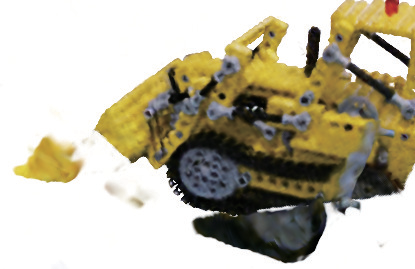
\includegraphics[width=0.118\textwidth]{figures/qualitative/s1_regnerf} &
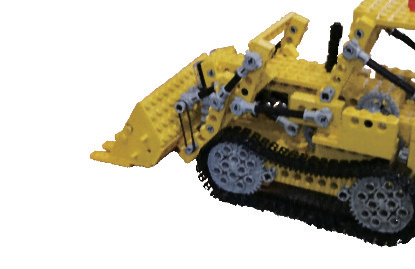
\includegraphics[width=0.118\textwidth]{figures/qualitative/s1_sparsenerf} &
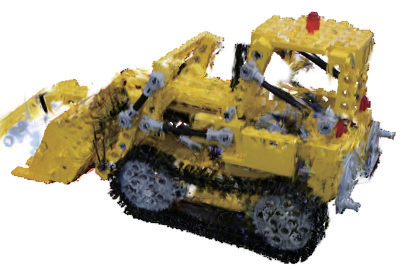
\includegraphics[width=0.118\textwidth]{figures/qualitative/s1_3dgs} &
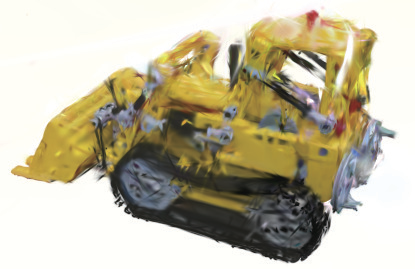
\includegraphics[width=0.118\textwidth]{figures/qualitative/s1_corgs} &
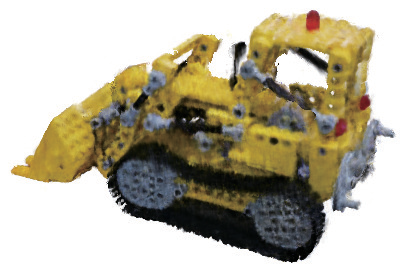
\includegraphics[width=0.118\textwidth]{figures/qualitative/s1_dropgaussian} &
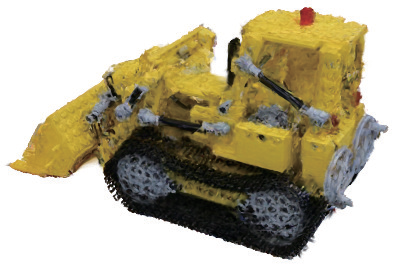
\includegraphics[width=0.118\textwidth]{figures/qualitative/s1_d2gs} &
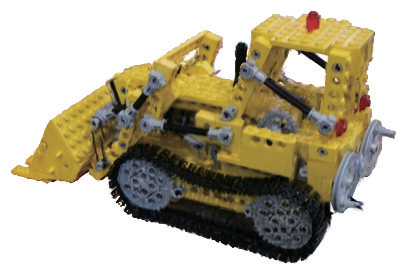
\includegraphics[width=0.118\textwidth]{figures/qualitative/s1_ours} &
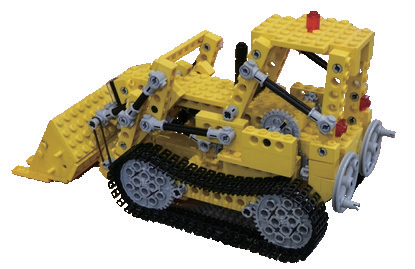
\includegraphics[width=0.118\textwidth]{figures/qualitative/s1_gt} \\[1pt]
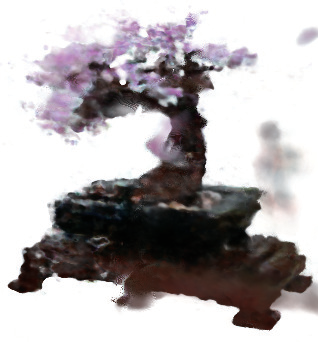
\includegraphics[width=0.118\textwidth]{figures/qualitative/s2_regnerf} &
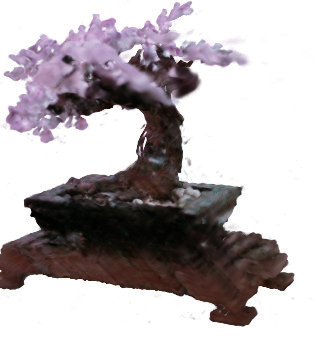
\includegraphics[width=0.118\textwidth]{figures/qualitative/s2_sparsenerf} &

\includegraphics[width=0.118\textwidth]{figures/qualitative/s2_3dgs} &

\includegraphics[width=0.118\textwidth]{figures/qualitative/s2_corgs} &

\includegraphics[width=0.118\textwidth]{figures/qualitative/s2_dropgaussian} &

\includegraphics[width=0.118\textwidth]{figures/qualitative/s2_d2gs} &

\includegraphics[width=0.118\textwidth]{figures/qualitative/s2_ours} &

\includegraphics[width=0.118\textwidth]{figures/qualitative/s2_gt} \\[1pt]
\makebox[0.118\textwidth]{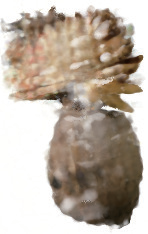
\includegraphics[height=0.127\textwidth]{figures/qualitative/s3_regnerf}} &
\makebox[0.118\textwidth]{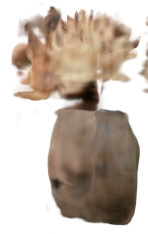
\includegraphics[height=0.127\textwidth]{figures/qualitative/s3_sparsenerf}} &
\makebox[0.118\textwidth]{
\includegraphics[height=0.127\textwidth]{figures/qualitative/s3_3dgs}} &
\makebox[0.118\textwidth]{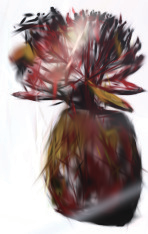
\includegraphics[height=0.127\textwidth]{figures/qualitative/s3_corgs}} &
\makebox[0.118\textwidth]{
\includegraphics[height=0.127\textwidth]{figures/qualitative/s3_dropgaussian}} &
\makebox[0.118\textwidth]{
\includegraphics[height=0.127\textwidth]{figures/qualitative/s3_d2gs}} &
\makebox[0.118\textwidth]{
\includegraphics[height=0.127\textwidth]{figures/qualitative/s3_ours}} &
\makebox[0.118\textwidth]{
\includegraphics[height=0.127\textwidth]{figures/qualitative/s3_gt}}
\end{tabular}
\caption{\label{fig:qualitative} Qualitative comparison under the 4-view sparse-input setting on Mip-NeRF 360. SynGS produces fewer floating artifacts and more complete structural boundaries than the compared methods.}
\end{figure}

\subsection{Ablation Study}
\label{sec:ablation}

Table~\ref{tab:ablation} \rev{presents an ablation analysis examining the contributions of the three components.} Unlike Table~\ref{tab:mip360}, which reports dataset-wide averages, the ablation is a separate protocol and is not the 4-view mean in Table~\ref{tab:mip360}.

% Table 3 — data from latex/消融实验/formatting-instructions-latex.tex (unchanged numbers)
\begin{table}[!htbp]
\centering
\caption{\label{tab:ablation} Ablation study of SynGS components. LPIPS$^{*}$ denotes LPIPS $\times 10^{2}$.}
\setlength{\tabcolsep}{2.5mm}
\renewcommand{\arraystretch}{1.05}
\small
\begin{tabular}{@{}cccccc@{}}
\toprule
\scriptsize Visual Hull Init & \scriptsize Depth Densification & \scriptsize Visibility Balancing$^{*}$ & SSIM$\uparrow$ & PSNR$\uparrow$ & LPIPS$^{*}$$\downarrow$ \\
\midrule
$\surd$  &              &              & 0.865  & 17.51  & 1.128  \\
$\surd$  & $\surd$      &              & 0.902  & 24.96  & 0.879  \\
$\surd$  & $\surd$      & $\surd$      & \textbf{0.943} & \textbf{26.18} & \textbf{0.609} \\
\bottomrule
\end{tabular}

\vspace{0.3em}
{\footnotesize $^{*}$Visibility Balancing denotes Dynamic Visibility Regularization (DVR).}
\end{table}


Visual Hull Initialization establishes the geometric baseline at 17.51~dB PSNR. Adding Depth Densification raises PSNR to 24.96~dB, the largest gain in the ablation. Adding DVR further improves the full configuration to 26.18~dB, with gains in SSIM and LPIPS.

\rev{The three configurations also clarify how the components contribute at different stages. The first configuration provides a reference for reconstruction using silhouette-derived geometry. The second incorporates additional depth-supported points before optimization, allowing the effect of geometric supplementation to be assessed against this reference. The third retains the enhanced initialization and introduces regularization during training. This sequence distinguishes the contribution of additional geometric information from that of the optimization strategy. Importantly, the ablation follows a separate evaluation protocol from the dataset-wide comparison in Table}~\ref{tab:mip360}\rev{. Its results should therefore be interpreted as comparisons between configurations within the ablation protocol, rather than as alternative estimates of the averages reported in Table}~\ref{tab:mip360}\rev{.}


\section{CONCLUSION}
\label{sec:conclusion}

We present SynGS for sparse-view 3DGS, combining \textbf{Visual Hull Initialization}, \textbf{VGGT-Guided Densification}, and \textbf{Dynamic Visibility Regularization} for more reliable initialization, geometry completion, and reduced sparse-view overfitting.
SynGS shows more pronounced improvements under highly sparse-view conditions, particularly in PSNR and SSIM with four or six input views. \rev{With nine input views, on Mip-NeRF 360, SynGS continues to outperform the compared approaches in terms of PSNR and SSIM, whereas its performance on LLFF is generally comparable to that of the other evaluated methods.} However, the additional geometry introduced during initialization incurs memory and computational overhead. \rev{Our future research will investigate ways to improve the efficiency of geometry augmentation, aiming to lower the associated computational and memory overhead without compromising reconstruction quality.}


\bibliography{references}
\bibliographystyle{spiebib}

\end{document}
